\documentclass{beamer}
\usepackage{../tut-slides}
\usepackage{../mathoperatorsAuD}

\usepackage{lmodern}
\usepackage{amsmath,amssymb}
\usepackage{wasysym}
\usepackage{stmaryrd}
\usepackage{enumerate}
%\usepackage[inline]{enumitem} 		%customize label
%\newcommand{\labelitemi}{\raisebox{1pt}{\scalebox{.9}{$\blacktriangleright$}}}
%\newcommand{\labelitemii}{$\vartriangleright$}
%\newcommand{\labelitemiii}{--}
\setbeamertemplate{itemize item}{\raisebox{1pt}{\scalebox{.9}{$\blacktriangleright$}}}
\setbeamertemplate{itemize subitem}{$\vartriangleright$}

\usepackage{booktabs}
\usepackage{tabularx}
\usepackage{tabu}
\newcommand*\head{\rowfont{\bfseries}}
\newcommand*{\tw}{\rowfont{\ttfamily}}
\renewcommand{\tabularxcolumn}[1]{>{\hspace{0pt}}m{#1}}
\usepackage{multirow}

\usepackage{cancel}

\usepackage{empheq}
\newcommand*\widefbox[1]{\fbox{\hspace{2em} #1 \hspace{2em}}}

\usepackage{tcolorbox}
\newtcolorbox{mymathbox}[1][]{colback=white, sharp corners, #1}

\usepackage{xcolor}
\usepackage{listings}
\lstset{numbers=left, 
	numberstyle=\tiny, 
	breaklines=true,
	backgroundcolor=\color{cdgray!20},
	numbersep=5pt,
	language=C,
	tabsize=2,
	basicstyle=\footnotesize\ttfamily,
	showstringspaces=false} 

\DeclareMathOperator{\ack}{\mathbf{ack}}
\usepackage{MnSymbol}

\newcommand{\col}[1]{\textcolor{cdpurple}{#1}}
\newcolumntype{R}[1]{>{\centering\arraybackslash}p{#1}}
\usepackage{tabularx}
\renewcommand{\tabularxcolumn}[1]{m{#1}}

\usepackage{qtree}
\usepackage[edges]{forest}

\newcommand{\lefttree}{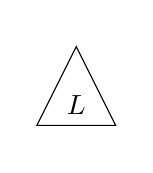
\begin{tikzpicture}
	\draw (0,0) node[anchor=north]{}
	-- (1,0) node[anchor=north]{}
	-- (.5,1) node[anchor=south]{}
	-- cycle;
	\draw (.5,.5) node[anchor=north]{$L$};
	\end{tikzpicture}}
\newcommand{\righttree}{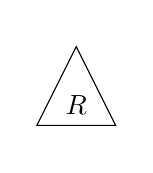
\begin{tikzpicture}
	\draw (0,0) node[anchor=north]{}
	-- (1,0) node[anchor=north]{}
	-- (.5,1) node[anchor=south]{}
	-- cycle;
	\draw (.5,.5) node[anchor=north]{$R$};
	\end{tikzpicture}}


\begin{document}	
	\title{Algorithmen und Datenstrukturen}
	\subtitle{Übung 11: AVL-Bäume \& Graphalgorithmen}
	\author{Eric Kunze}
	\email{eric.kunze@mailbox.tu-dresden.de}
	\city{TU Dresden}
%	\institute{Lehrstuhl für Grundlagen der Programmierung}
	\titlegraphic{\includegraphics[width=2cm]{../TUD-white.pdf}}
	\date{16.01.2020}

	\maketitle


%%%%%%%%%%%%%%%%%%%%%%%%%%%%%%%%%%%%%%%%%%%%%%%%%%%%%%%%%%%%%%%%%%%%%%%%%%%%%



%%%%%%%%%%%%%%%%%%%%%%%%%%%%%%%%%%%%%%%%%%%%%%%%%%%%%%%%%%%%%%%%%%%%%%%%%%%%%%%%%%%

\section{Breiten- und Tiefensuche}

\begin{frame} \frametitle{Aufgabe 2}
	\centering
	\includegraphics[height=15em]{./tut11_task2-graph.pdf}
\end{frame}

\begin{frame} \frametitle{Aufgabe 2 --- Teil (a)}
	Es gibt $5$ verschiedene depth-first-trees, z.B.:
	
	\includegraphics[width=\linewidth]{./tut11_task2-dft.pdf}
\end{frame}

\begin{frame} \frametitle{Aufgabe 2 --- Teil (b)}
	Es gibt $5$ verschiedene breadth-first-trees, z.B.:
	
	\includegraphics[width=\linewidth]{./tut11_task2-bft.pdf}
\end{frame}

%%%%%%%%%%%%%%%%%%%%%%%%%%%%%%%%%%%%%%%%%%%%%%%%%%%%%%%%%%%%%%%%%%%%%%%%%%%%%%%%%%%

\section{Floyd-Warshall-Algorithmus}

\begin{frame} \frametitle{Floyd-Warshall-Algorithmus}
	\begin{itemize}
		\item (gewichteter) Graph $G = (V,E,c)$ mit Weglängen $c$ und ohne Schlingen
		\item \textbf{Ziel}: kürzeste Wege von beliebigem Startknoten zu beliebigem Zielknoten
		\item oBdA: $V = \menge{1, \dots, n}$
		\item $P_{u,v} =$ Menge aller Wege von $u$ nach $v$
		\item $D_G (u,v) = \begin{cases}
		\min\menge{c_p : p \in P_{u,v}} & \text{wenn } P_{u,v} \neq \emptyset \\
		\infty & \text{sonst}
		\end{cases}$
		\item $P^{(k)}_{u,v} =$ Menge aller Wege von $u$ nach $v$, deren innere Knoten in $\menge{\ell : 1 \le \ell \le k}$ liegen
		\item $D_G^{(k)} (u,v) = \begin{cases}
		\min\menge{c_p : p \in P_{u,v}^{(k)}} & \text{wenn } P_{u,v}^{(k)} \neq \emptyset \\
		\infty & \text{sonst}
		\end{cases}$
		\item Es gilt $P^{(n)}_{u,v} = P_{u,v}$ und somit $D_G^{(n)} = D_G$
	\end{itemize}
\end{frame}

\begin{frame} \frametitle{Floyd-Warshall-Algorithmus}
	\begin{itemize}
		\item modifizierte Adjazenzmatrix $mA_G = \min\menge{A_G, \mathbf{0}_n} = \begin{cases}
		c(u,v) & \text{wenn } u \neq v, (u,v) \in E \\
		0 & \text{wenn } u = v \\
		\infty & \text{sonst}
		\end{cases}$
		\item \textbf{Initialisierung}: $D_G^{(0)} = mA_G$
		\item \textbf{Rekursion}:
		\begin{equation*}
			\boxed{D_G^{(k+1)}(u,v) = \min\menge{D_G^{(k)}(u,v) , D_G^{(k)}(u,k+1) + D_G^{(k)}(k+1,v)}}
		\end{equation*}
	\end{itemize}
\end{frame}
\begin{frame} \frametitle{Aufgabe 3}
	\begin{minipage}{\dimexpr0.42\linewidth-\fboxrule-\fboxsep}
		\includegraphics[height=13em]{./tut11_task3-graph.pdf}
	\end{minipage}
	\pause
	\begin{minipage}{\dimexpr0.58\linewidth-\fboxrule-\fboxsep}
		\small
		$mA_G = \begin{pmatrix}
		0      & \infty & 3      & \infty & \infty & \infty & \infty \\
		8      & 0      & \infty & 2      & \infty & \infty & \infty \\
		\infty & \infty & 0      & \infty & \infty & \infty & \infty \\
		4      & \infty & 8      & 0      & \infty & 3      & 6      \\
		\infty & 4      & \infty & 7      & 0      & \infty & 15     \\
		\infty & \infty & 3      & \infty & \infty & 0      & 2      \\
		\infty & \infty & \infty & \infty & \infty & \infty & 0
		\end{pmatrix}$
	\end{minipage}
\end{frame}

\begin{frame} \frametitle{Aufgabe 3 --- Teil (b)}
	\begin{equation*}
		D_G^{(2)} = \begin{pmatrix}
		0      & \infty & 3      & \infty & \infty & \infty & \infty \\
		8      & 0      & \textcolor{cdpurple}{11}     & 2      & \infty & \infty & \infty \\
		\infty & \infty & 0      & \infty & \infty & \infty & \infty \\
		4      & \infty & \textcolor{cdpurple}{7}     & 0      & \infty & 3      & 6      \\
		\textcolor{cdgreen}{12}     & 4      & \textcolor{cdgreen}{15}     & \textcolor{cdgreen}{6}      & 0      & \infty & 15     \\
		\infty & \infty & 3      & \infty & \infty & 0      & 2      \\
		\infty & \infty & \infty & \infty & \infty & \infty & 0
		\end{pmatrix}
	\end{equation*}
	d.h. es ändern sich folgende Einträge:
	\begin{equation*}
		\underbrace{\textcolor{cdpurple}{(4,3,7), (2,3,11)}}_{\text{aus } D_G^{(1)}}, \underbrace{\textcolor{cdgreen}{(5,3,15), (5,1,12), (5,4,6)}}_{\text{aus } D_G^{(2)}} 
	\end{equation*}
\end{frame}

\begin{frame} \frametitle{Aufgabe 3 --- Teil (c)}
	Für $k \in \menge{4,6}$, d.h. durch Zulassen der Knoten $4$ und $6$ als innere Knoten eines Weges, erreichen wir eine Verbesserung. Dagegen sind die Knoten $3$ und $7$ \textit{Senken}, d.h. es bringt nichts, diese zu besuchen, weil wir nicht wieder weg kommen. Ebenso bringt uns der Knoten $5$ als \textit{Quelle} keine Verbesserung, weil wir diesen gar nicht erreichen können.
	Somit gilt also
	\begin{equation*}
		D_G^{(2)} = D_G^{(3)} \qquad D_G^{(4)} = D_G^{(5)} \qquad D_G^{(6)} = D_G^{(7)}
	\end{equation*}
	und wir müssen lediglich $D_G^{(4)}$ sowie $D_G^{(6)}$ explizit berechnen.
\end{frame}

\begin{frame} \frametitle{Aufgabe 3 --- Teil (d)}
	\small
	\begin{equation*}
	\begin{aligned}
		D_G^{(4)} &= \begin{pmatrix}
		0      & \infty & 3      & \infty & \infty & \infty & \infty \\
		\alert{6}      & 0      & \alert{9}     & 2      & \infty & \alert{5} & \alert{8} \\
		\infty & \infty & 0      & \infty & \infty & \infty & \infty \\
		4      & \infty & 11     & 0      & \infty & 3      & 6      \\
		\alert{10}     & 4      & \alert{13}     & 6      & 0      & \alert{9} & \alert{12}     \\
		\infty & \infty & 3      & \infty & \infty & 0      & 2      \\
		\infty & \infty & \infty & \infty & \infty & \infty & 0
		\end{pmatrix}
		= D_G^{(5)} \\
		D_G^{(6)} &= \begin{pmatrix}
		0          & \infty & 3          & \infty & \infty & \infty & \infty \\
		6          & 0      & \alert{8}  & 2      & \infty & 5      & \alert{7} \\
		\infty     & \infty & 0          & \infty & \infty & \infty & \infty \\
		4          & \infty & \alert{6}  & 0      & \infty & 3      & \alert{5}     \\
		10         & 4      & \alert{12} & 6      & 0      & 9      & \alert{11}     \\
		\infty     & \infty & 3          & \infty & \infty & 0      & 2      \\
		\infty     & \infty & \infty     & \infty & \infty & \infty & 0
		\end{pmatrix}
		= D_G^{(7)} = D_G
	\end{aligned}
	\end{equation*}
\end{frame}
\end{document}